\section{Μέθοδοι και Χρονοδιάγραμμα Υλοποίησης}
\begin{frame}
	\frametitle{Μέθοδοι και Χρονοδιάγραμμα Υλοποίησης}

	\centering
	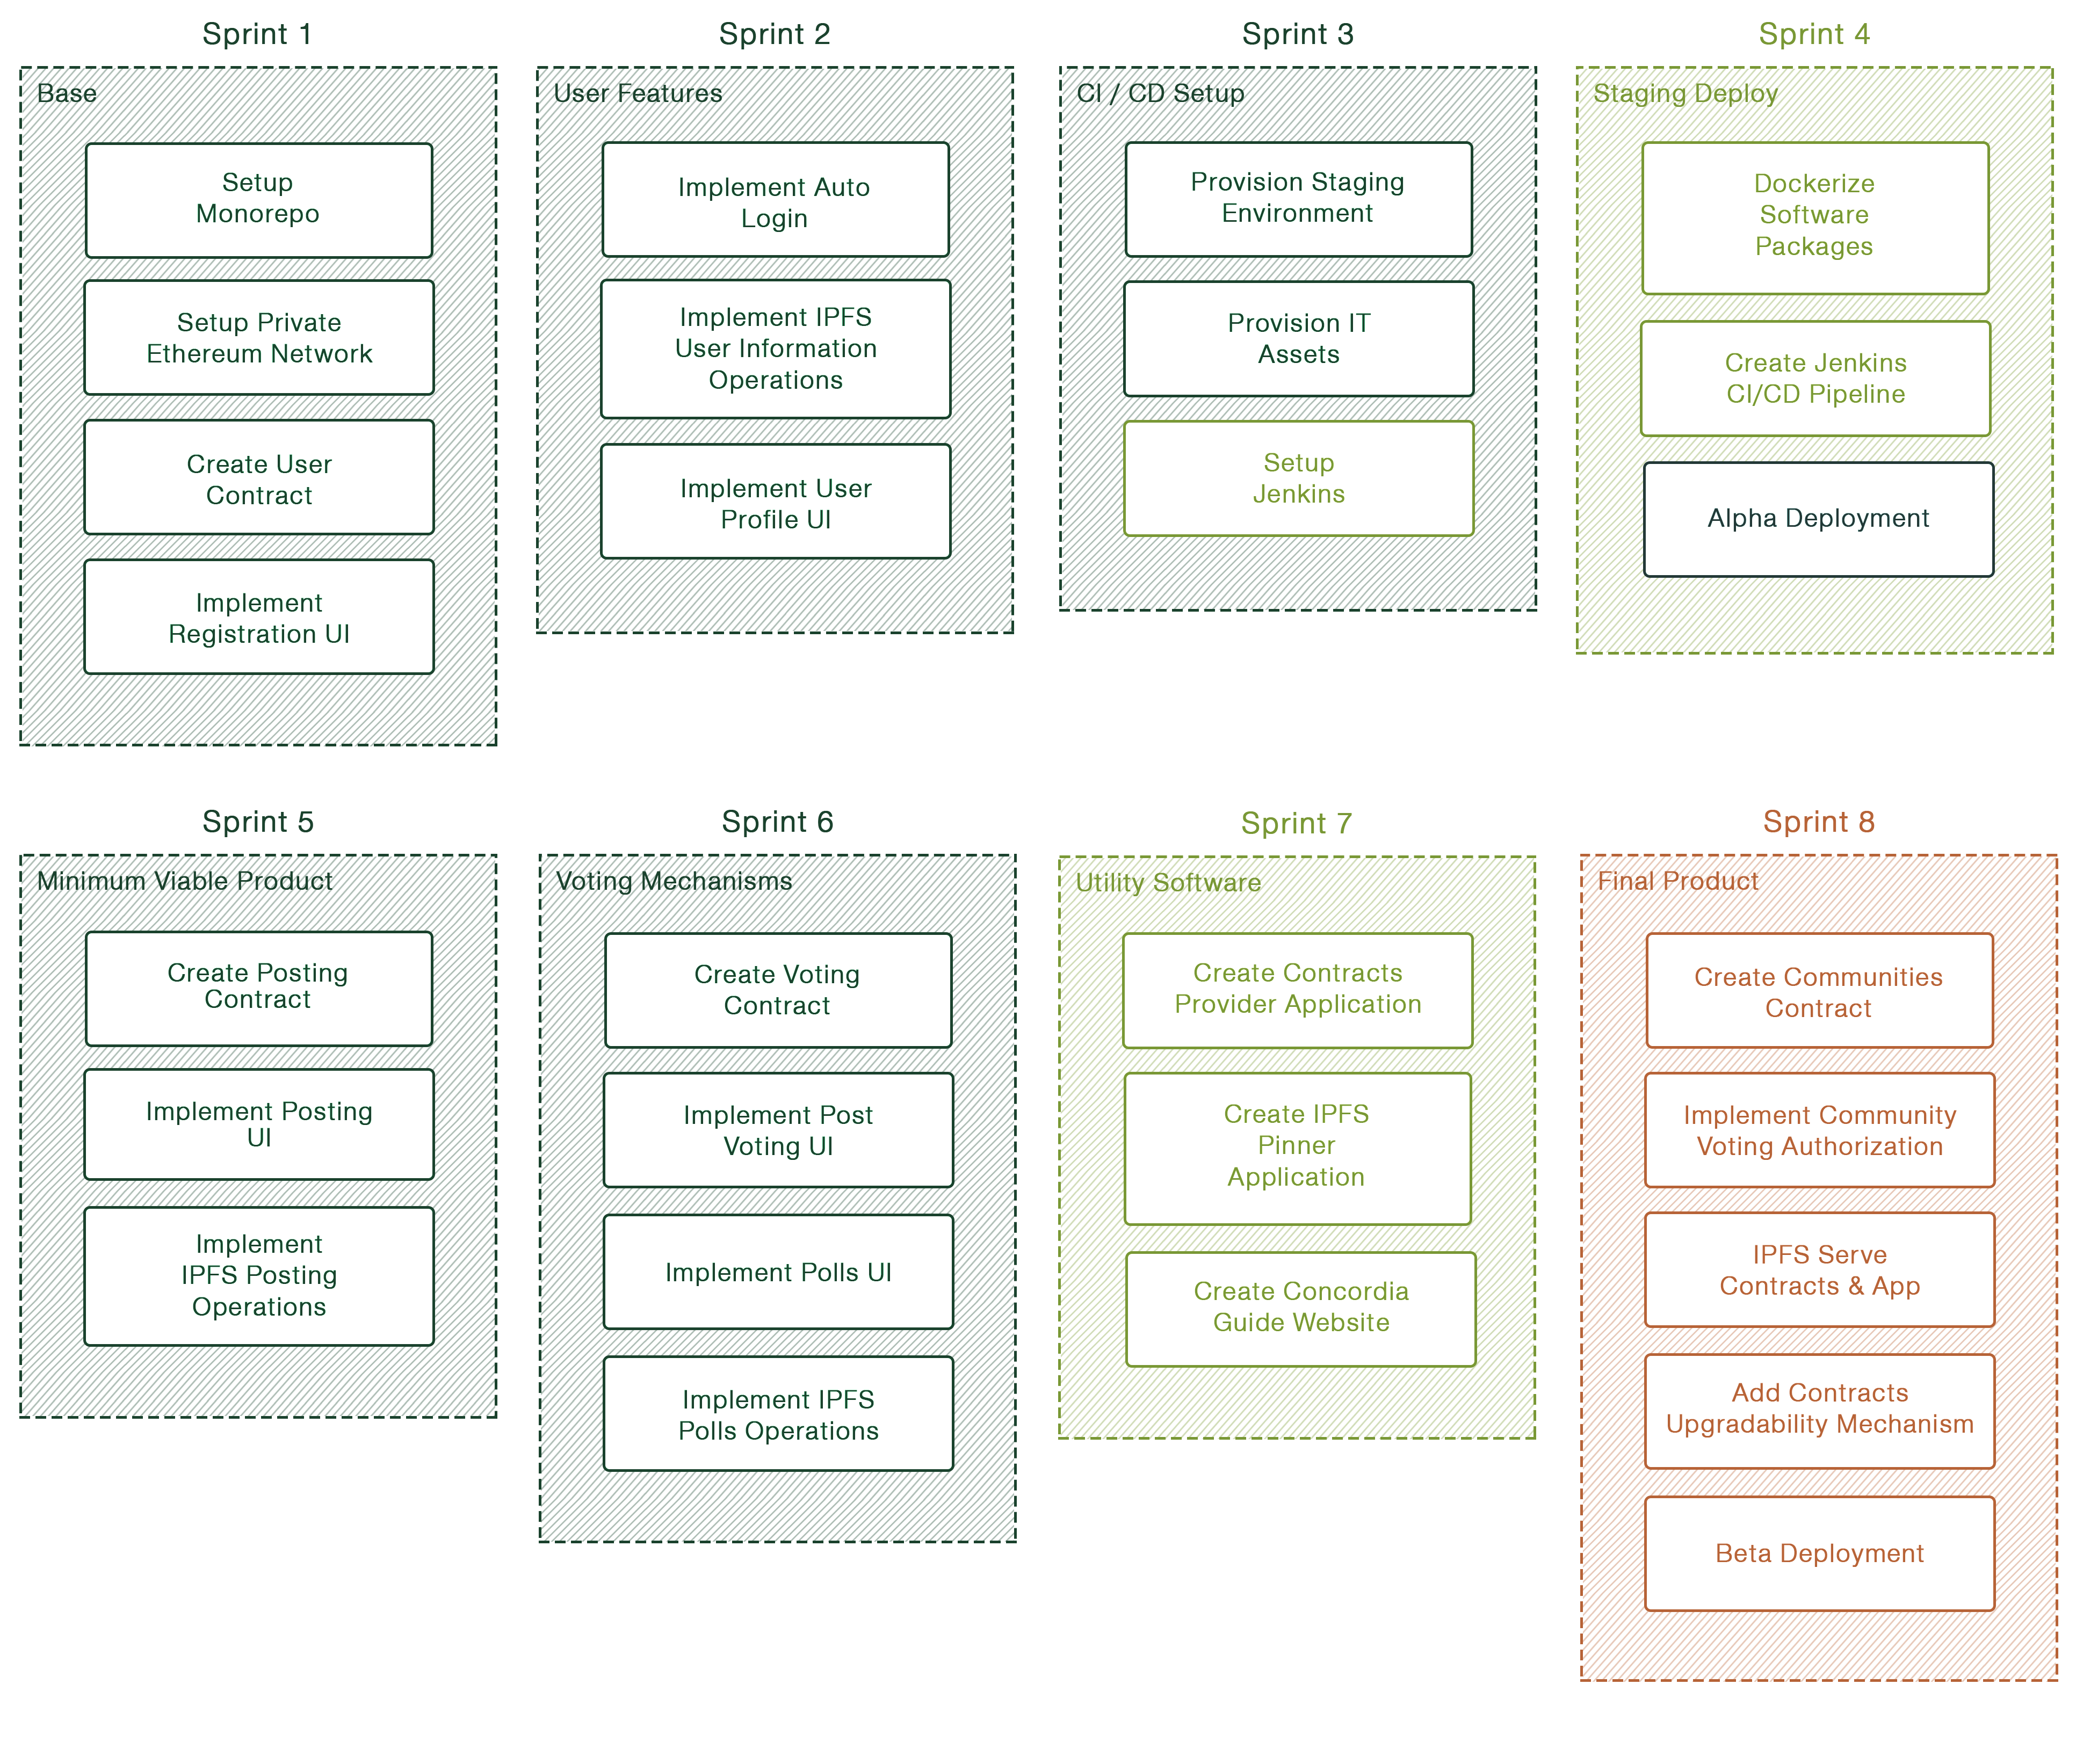
\includegraphics[width=.82\textwidth]{assets/figures/implementation-sprints.png}
\end{frame}

\note{
	Σε αυτό το μέρος της παρουσίασης θα αναλύσουμε τις μεθόδους που χρησιμοποιήθηκαν κατά την ανάπτυξη της εφαρμογής και τον χρονοπρογραμματισμό που έγινε.

	Τόσο η σχεδίαση όσο και η ανάπτυξη της εφαρμογής ακολούθησαν τις σύγχρονες μεθόδους Agile development.

	Το συνολικό έργο χωρίστηκε σε tasks. Τα tasks είναι αυτόνομα μέρη υλοποίησης που λύνουν ένα μικρό υπο-πρόβλημα της συνολικής σχεδίασης. Δημιουργήθηκαν οχτώ ομάδες οι οποίες αναφέρονται σε διακριτούς στόχους της πλατφόρμας και ομαδοποιούν τα tasks τα οποία συνεισφέρουν στον στόχο αυτό. Κάθε ομάδα υλοποιήθηκε διαδοχικά καταλαμβάνοντας τρεις βδομάδες ανάπτυξης.

	Για τις ανάγκες της υλοποίησης, έγινε επίσης χρήση του συστήματος CI-CD Jenkins. Το Jenkins είναι ένα αυτοματοποιημένο σύστημα ενσωμάτωσης, ελέγχου και ολοκλήρωσης λογισμικού.
}
